\documentclass[letterpaper,11pt]{./templates/texMemo} % Set the paper size (letterpaper, a4paper, etc) and font size (10pt, 11pt or 12pt)

\usepackage{graphicx}
\graphicspath{ {../img/} }
\usepackage[parfill]{parskip} % Adds spacing between paragraphs
\setlength{\parindent}{0pt} % Indent paragraphs
\usepackage{float}

%----------------------------------------------------------------------------------------
%   MEMO INFORMATION
%----------------------------------------------------------------------------------------

\memoto{Industrial Consultant} % Recipient(s)

% Setup of the document
\memosubject{Project Brief}
\memofrom{Team 14 - Daniel DeHoog, T.J. DeVries,
    Paul Griffioen, Ryan Siekman}

\memodate{February 29, 2016}

% Now the writing of the document can begin
\begin{document}

\maketitle 

\section{Team Members}

% Include the team members
\centerline{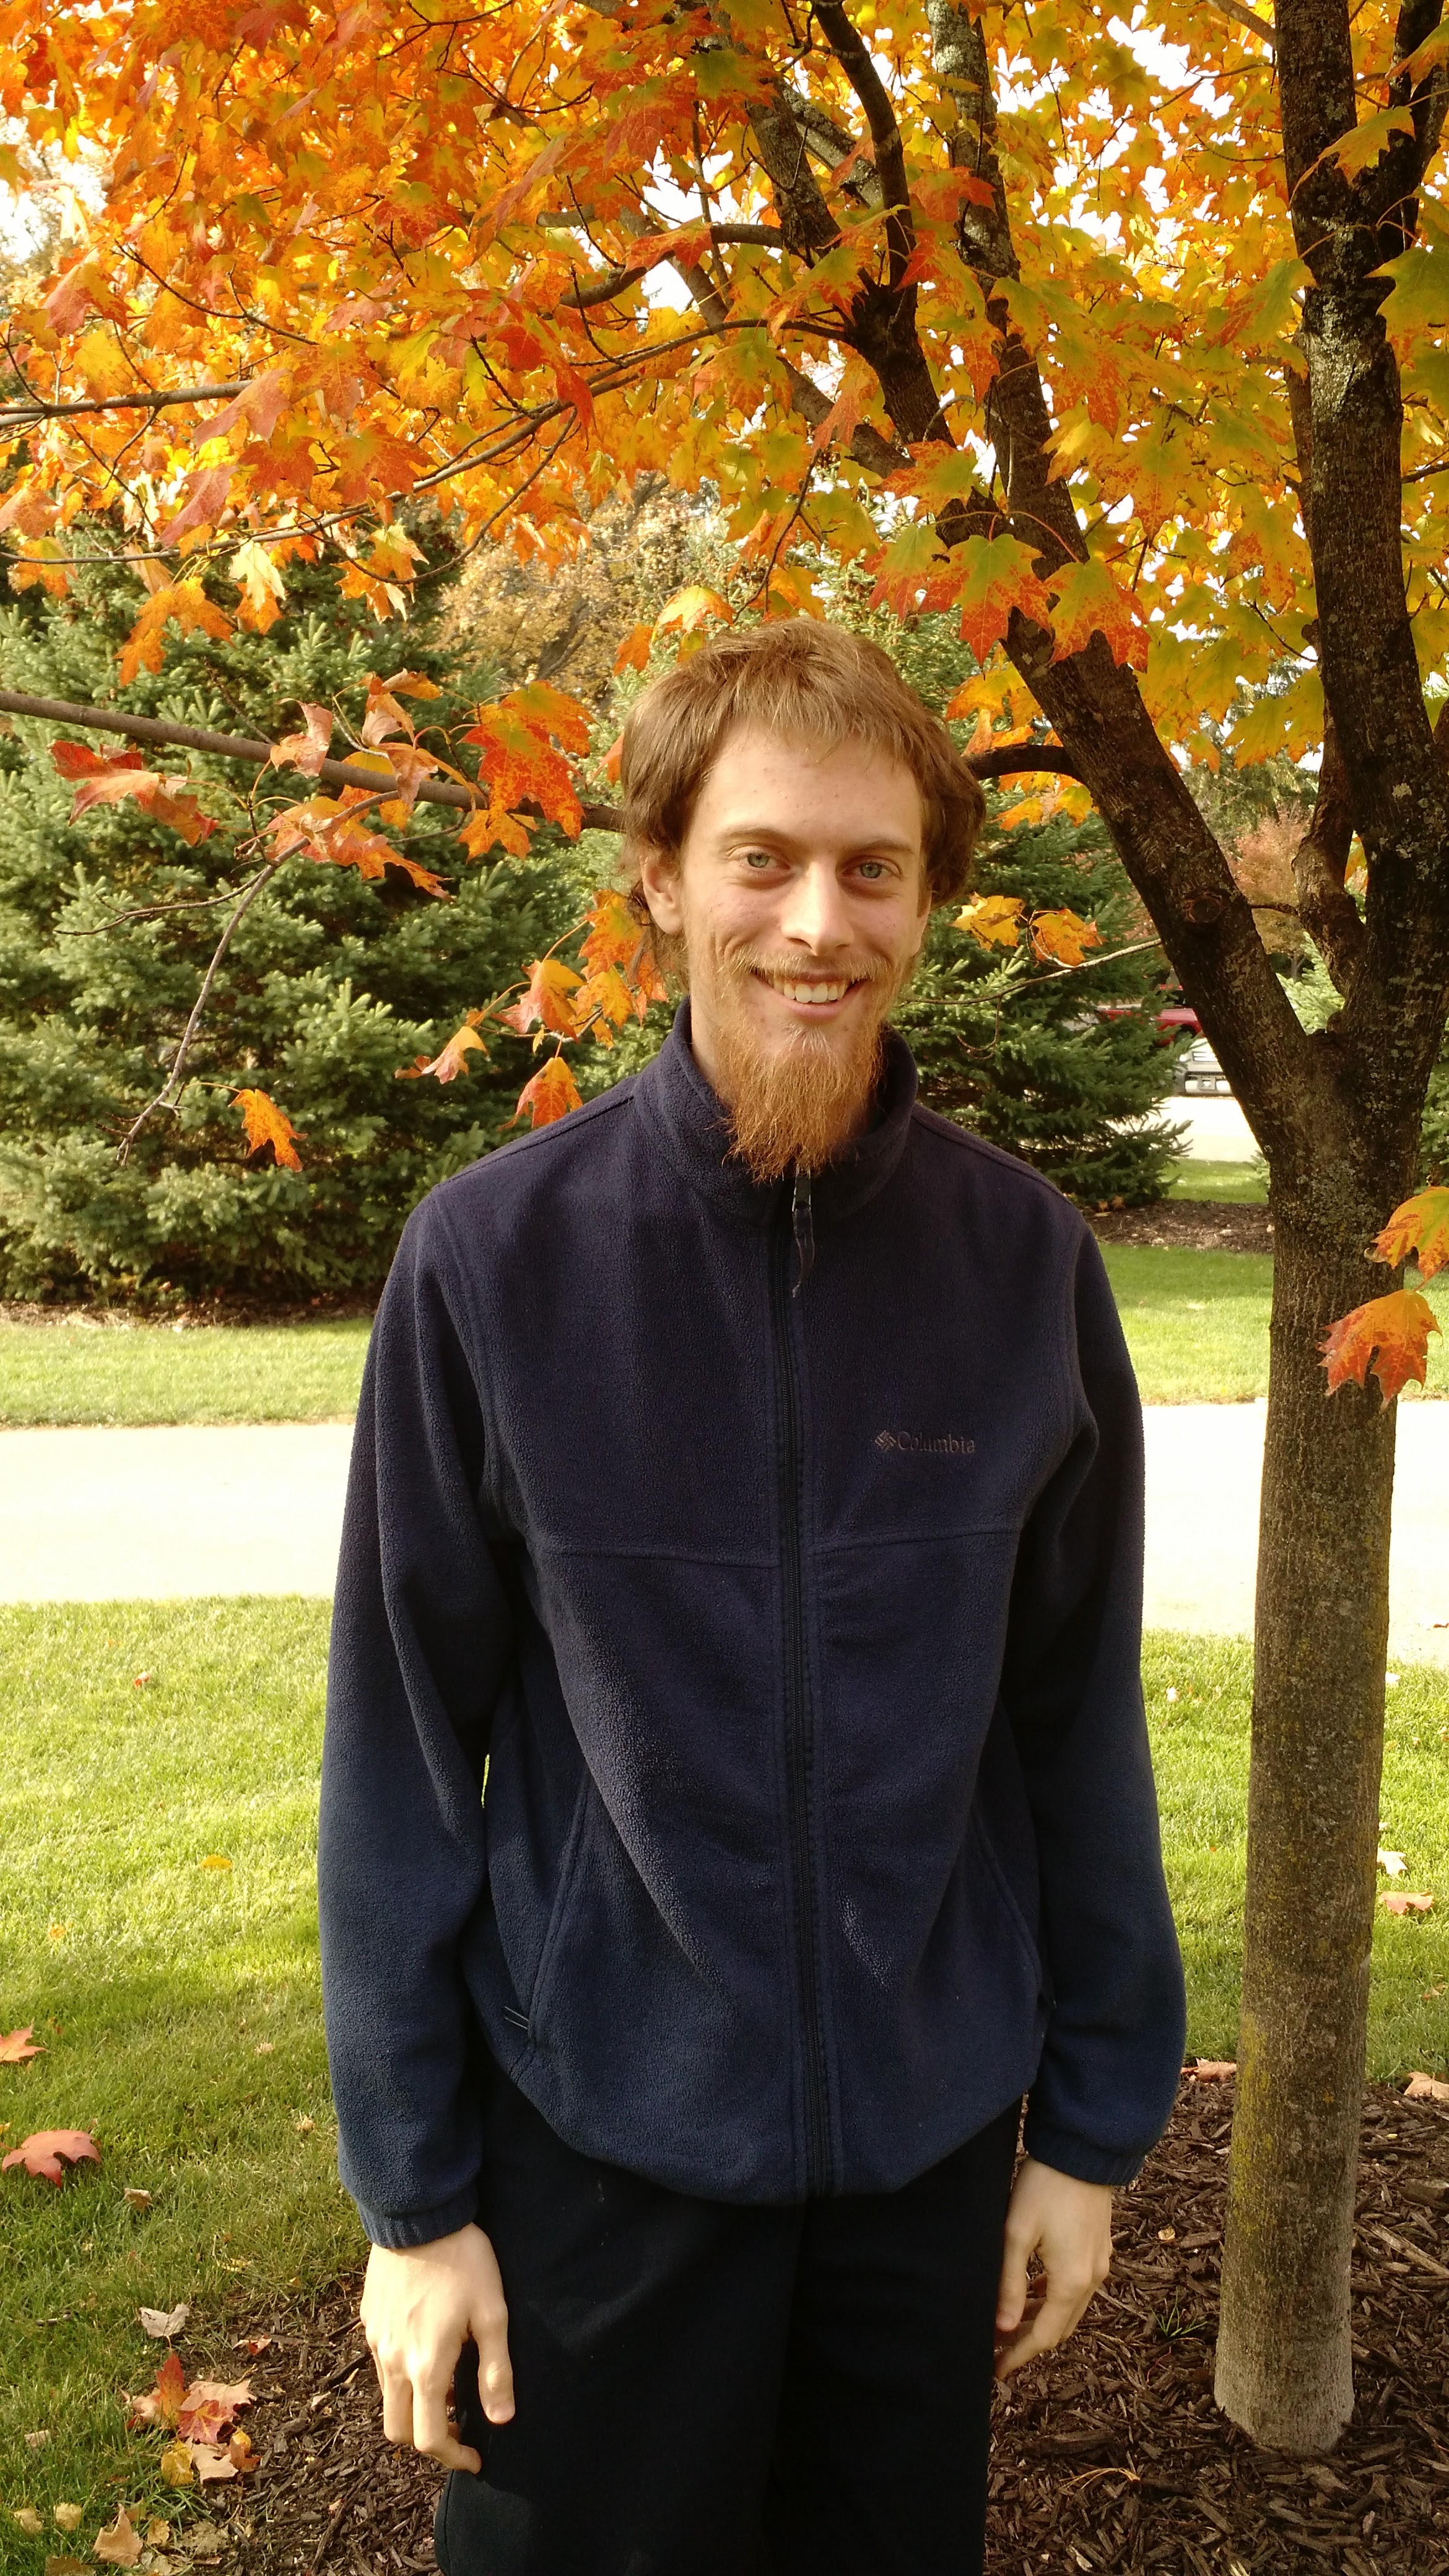
\includegraphics[width=0.25\textwidth]{dan.jpg} 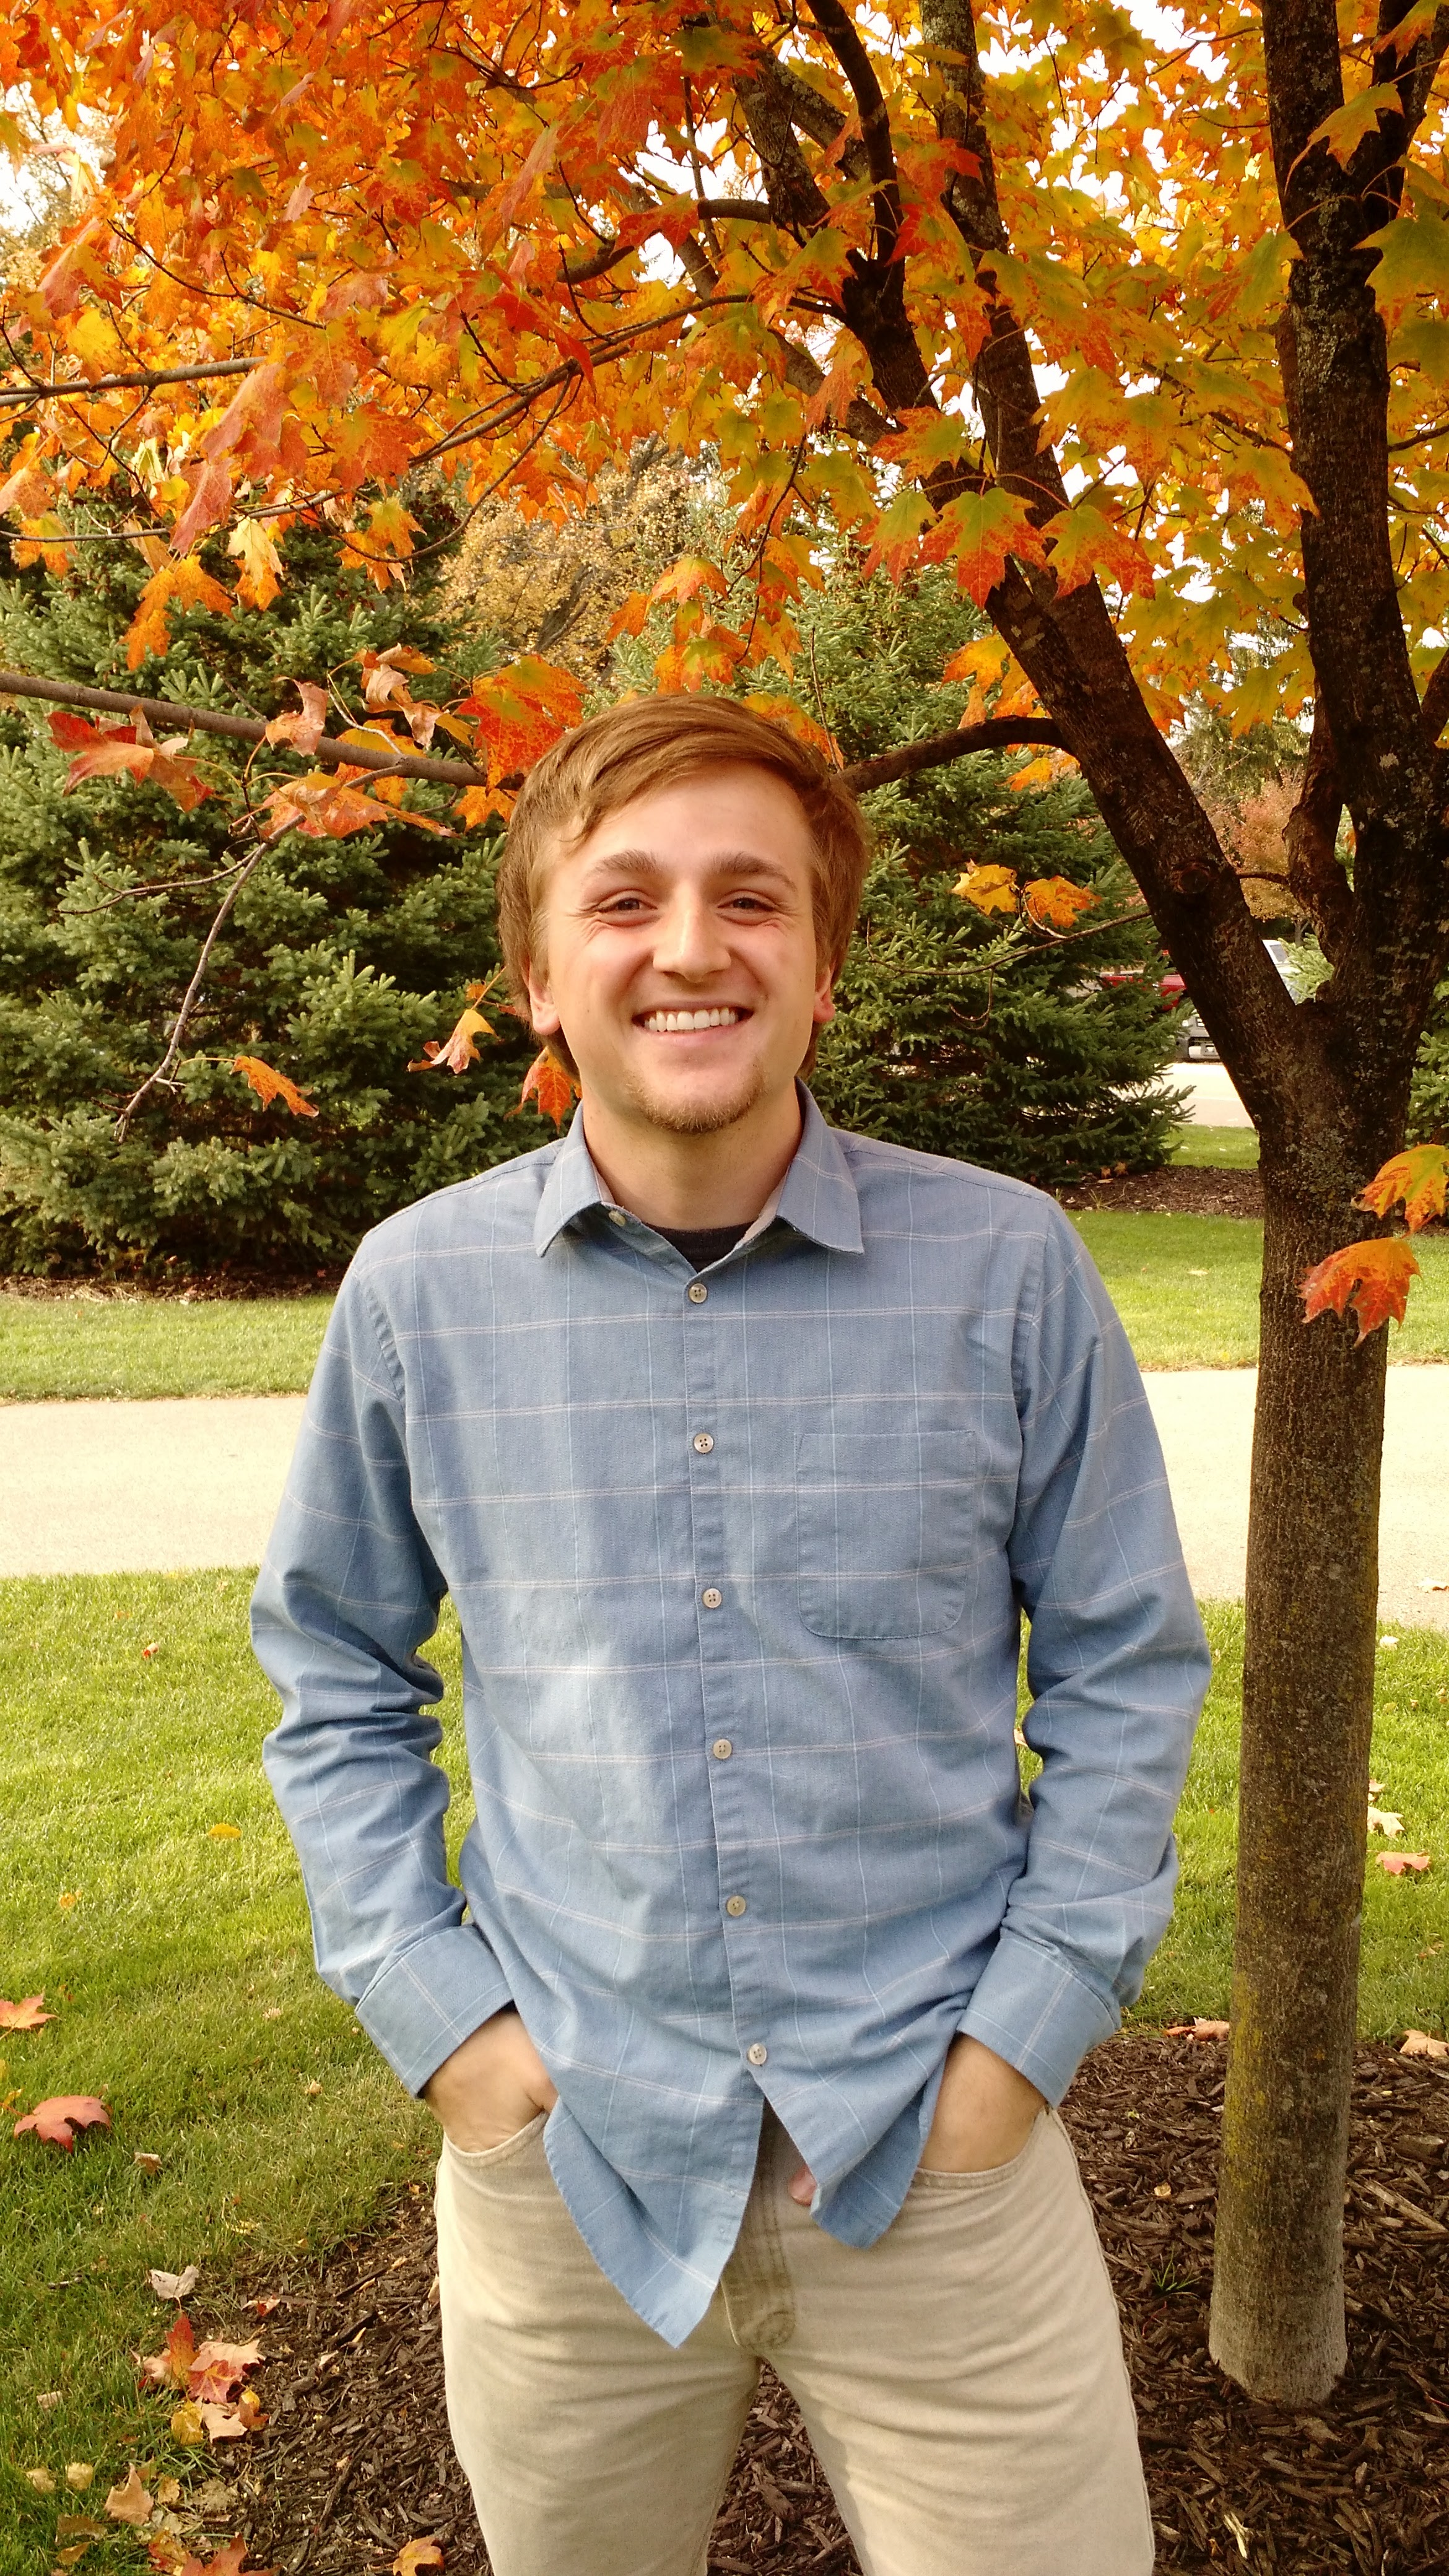
\includegraphics[width=0.25\textwidth]{tj.jpg} 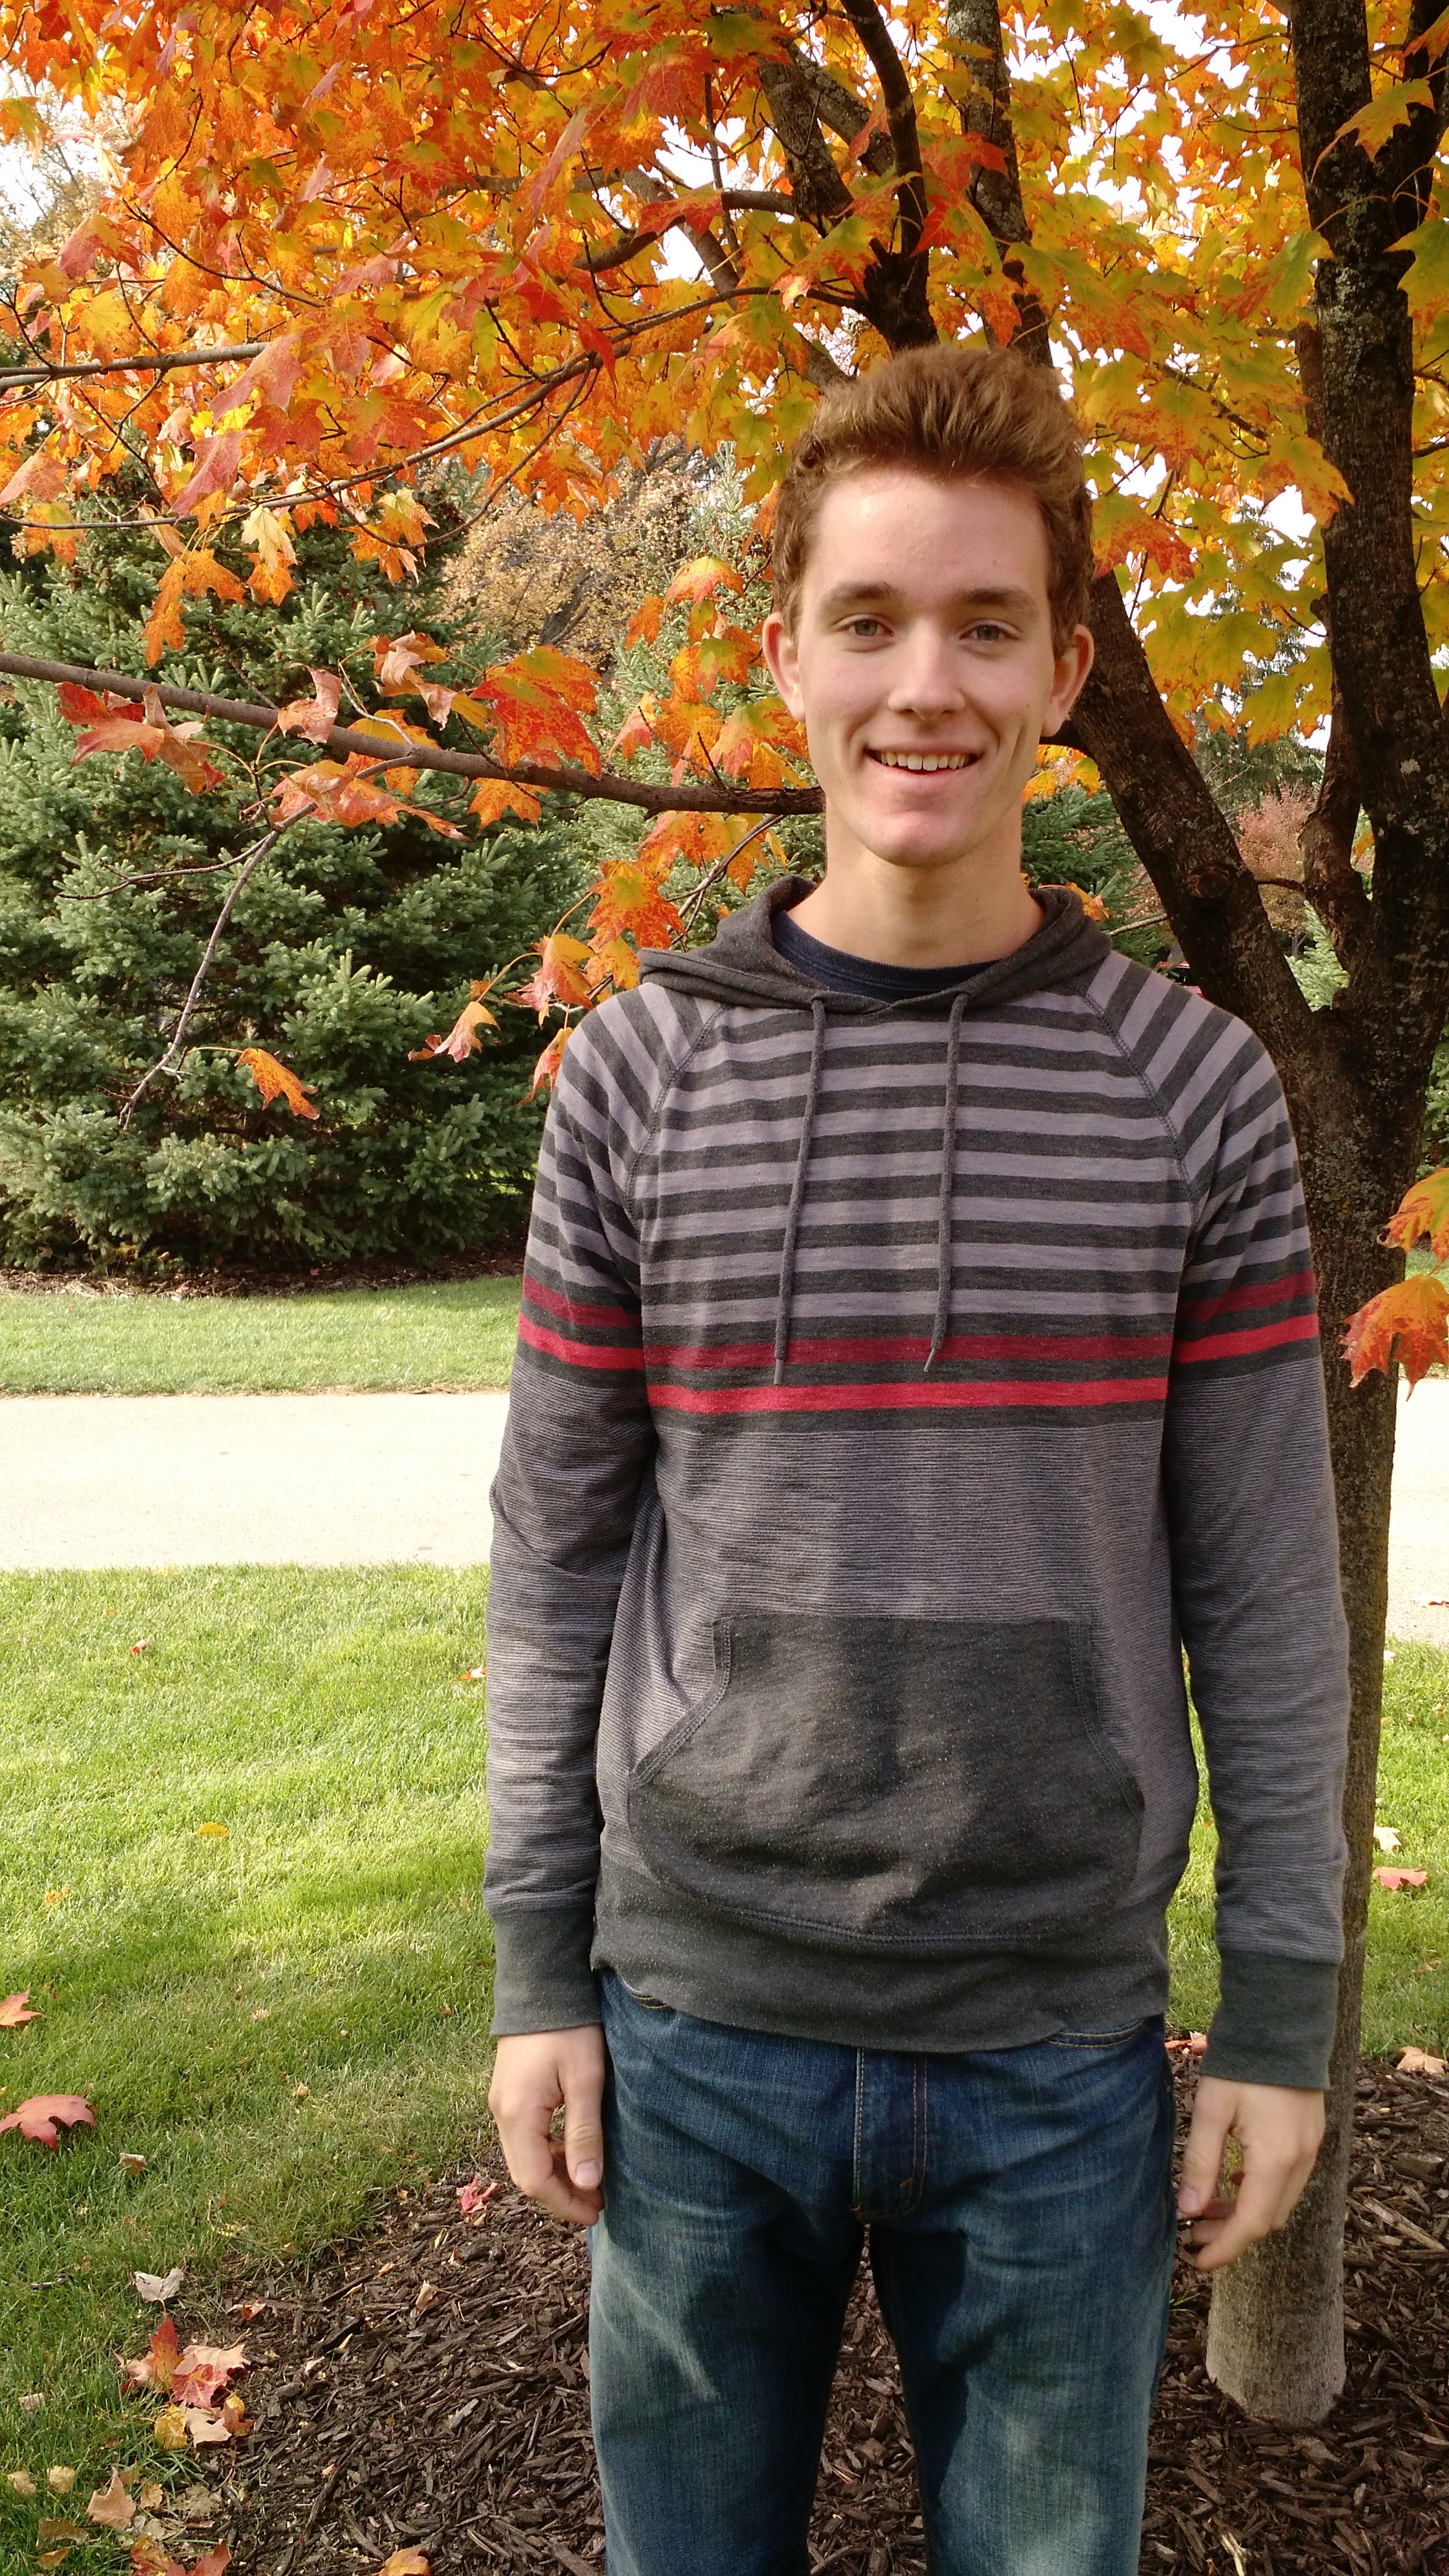
\includegraphics[width=0.25\textwidth]{paul.jpg} 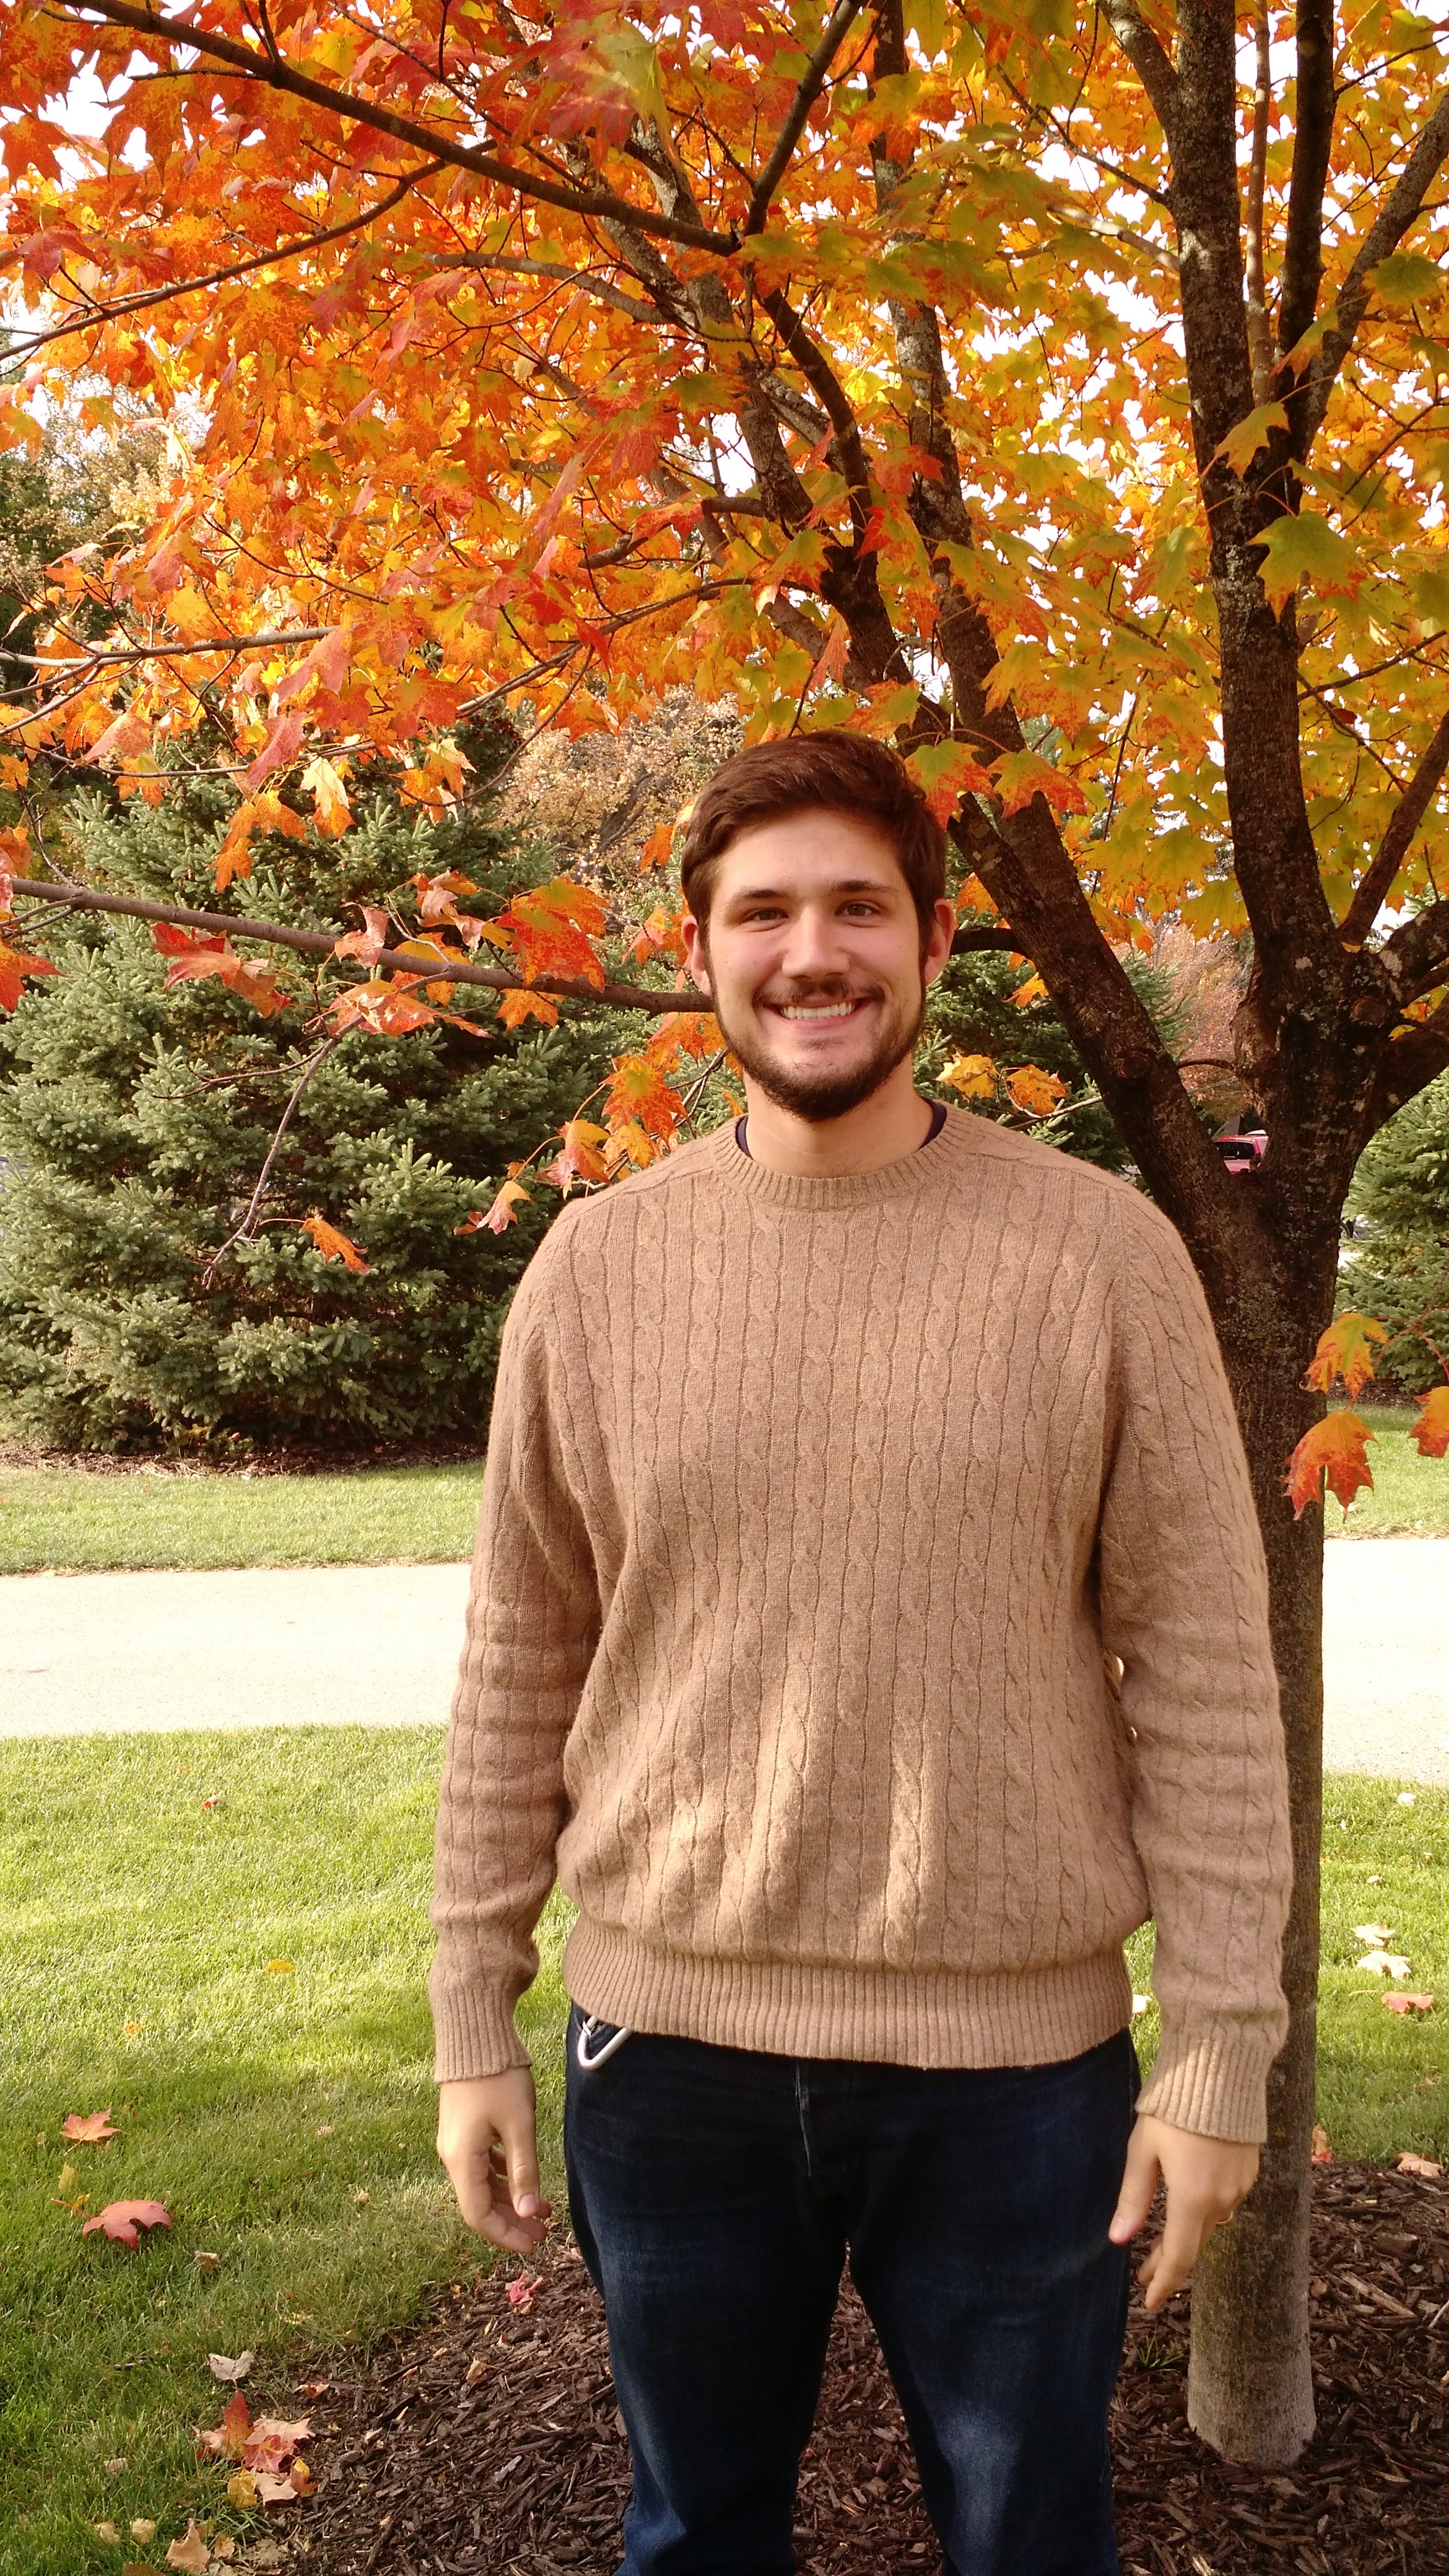
\includegraphics[width=0.25\textwidth]{ryan.jpg}}
\centerline{Daniel DeHoog, TJ DeVries, Paul Griffioen, Ryan Siekman}

\section{Project Description}

Create a system that will allow people, both clients and administrators, to interact with gyms in a modern and smart way. This system will allow users to view what machines are currently open, and it will also allow users to reserve systems for personal use. The system will also provide gym administrators with the ability to understand more clearly what machines get used, along with how often and when they are used.

\section{Project Requirements}

The following subsections list the project requirements, which are divided into system requirements and hardware requirements. Necessary requirements are listed as is, whereas optional requirements are presented in brackets.

\subsection{System Requirements}

    \begin{itemize}
    \item{\textbf{Generic}}
    \begin{itemize}
        \item{Ability to install the system in a typical existing gym}
        \item{Transferable - ability to transfer sensors and displays from one type of machine/equipment to another}
        \item{Ability to install each sensor and each display on (most) any type of stationary equipment}
        \item{[Ability to install sensors on free weights, weight sets, and other moving equipment]}
    \end{itemize}

    \item{\textbf{General}}
    \begin{itemize}
        \item{Ability to run continuously for 24 hours without crashing}
        \item{Price is small enough that existing gyms would be willing to invest in buying it}
        \item{Ability for gyms to only use parts of the system if desired}
        \item{Ability to add or remove parts after initial setup and installation}
    \end{itemize}

    \item{\textbf{Accessibility}}
    \begin{itemize}
        \item{Data should be accessible via a web interface (mobile device and personal computer)}
        \item{Detailed data about equipment use should be accessible for gym managers}
        \item{[Fitness data should be available for personal use]}
    \end{itemize}

    \item{\textbf{User-Friendly}}
    \begin{itemize}
        \item{Sensors should not impede use of machinery or weights}
        \item{Web interface and mobile application should be simple and easy to use}
    \end{itemize}

    \item{\textbf{Reservation System}}
    \begin{itemize}
        \item{Organized according to machine, user, and time}
        \item{Implement rules about making reservations and canceling them to protect against system abusers}
        \item{Reservation information for a specific machine should appear on that machine's display}
        \begin{itemize}
            \item{Allow user to interact with the display to edit the reservation}
        \end{itemize}
        \item{No power supply required for reservation display or sensors}
        \item{[Bulk reservations (over multiple periods of time)]}
        \item{[Electronic calendar integration]}
    \end{itemize}

    \item{\textbf{Real-Time Updates}}
    \begin{itemize}
        \item{Real-time updates of which machines are currently being used}
        \begin{itemize}
            \item{Each update occurs within one minute}
        \end{itemize}
        \item{Based on data acquired from sensors, not data used from reservation system}
    \end{itemize}

    \item{\textbf{Central Management}}
    \begin{itemize}
        \item{Smart hub, located within the gym, must collect data from the sensors and communicate data to the displays}
        \item{Data will be collated by a central server}
        \begin{itemize}
            \item{Central server will manage the reservation system, web interface, and mobile application}
        \end{itemize}
        \item{[Smart hub will cache daily schedules for sending to the displays in case internet connection is lost]}
    \end{itemize}
    \end{itemize}

\subsection{Hardware Requirements}

    \begin{itemize}
    \item{\textbf{Sensors}}
    \begin{itemize}
        \item{Used to determine whether or not a machine is in use}
        \item{Must be movement sensors (accelerometer, gyroscope, or magnetometer) on a single board}
        \item{Long battery life, on the order of years}
        \item{Small size (less than 5 in$^2$)}
        \item{Possess network capabilities with the ability to form a mesh network, where the sensors can communicate with and pass data to one another}
        \item{Ability to make strong yet removable physical connections to each machine}
    \end{itemize}
    
    \item{\textbf{Display Interfaces}}
    \begin{itemize}
        \item{Used to display machine reservations}
        \item{Long battery life, on the order of months}
        \item{Display information, such as a name and reservation time, in a user-friendly manner}
        \item{Ability to handle sweat that may fall on the display}
        \item{Possess network capabilities with the ability to form a mesh network, where the displays can communicate with and pass data to one another}
        \item{Display must be compatible with the mesh network}
        \item{Relatively small (approx. 2 in by 3 in) with at least 2 push buttons and 1 LED for making reservations}
    \end{itemize}
    
    \item{\textbf{Hub}}
    \begin{itemize}
        \item{A small yet powerful computer (raspberry pi) placed within the gym}
        \item{Capable of running multiple operating systems (Linux and Windows)}
        \item{Ethernet connection for reliable internet connection}
        \item{Ability to communicate with the mesh network of sensors and displays (wifi, zigbee, bluetooth)}
        \item{[Ability to turn on and off sensors and displays to save energy]}
    \end{itemize}
    
    \item{\textbf{Server}}
    \begin{itemize}
        \item{A reliable computer with the ability to communicate with the hub}
        \item{Host the website and mobile application that users employ for reservations and seeing which machines are currently in use}
        \item{Store the database of information for reservations and data collected from the sensors}
    \end{itemize}
    \end{itemize}

\section{Design Decisions}
Many of the design decisions for this project are based on the hardware chosen. The following hardware has been chosen to be implemented in the project, either for testing or for final implementation:
\begin{itemize}
\item{TI SensorTag, featuring the CC2650 wireless MCU}
\item{TI SimpleLink Multi-Standard SensorTag Development Kit}
\item{TI SimpleLink SensorTag DevPack}
\item{2.7-inch Sharp Memory LCD}
\item{Raspberry Pi 1, Model B+}
\item{Raspberry Pi 2, Model B}
\item{TI CC Debugger for the CC2531 USB Dongle}
\item{CC2531 USB Evaluation Module Kit}
\item{5-Port TP-Link Desktop Switch}
\end{itemize}

Figure \ref{fig:general_overview} depicts a UML diagram of the system overview that is currently being implemented in the project. At this time, there are no significant project issues that must be addressed.

\begin{figure}[H]
    \centering
    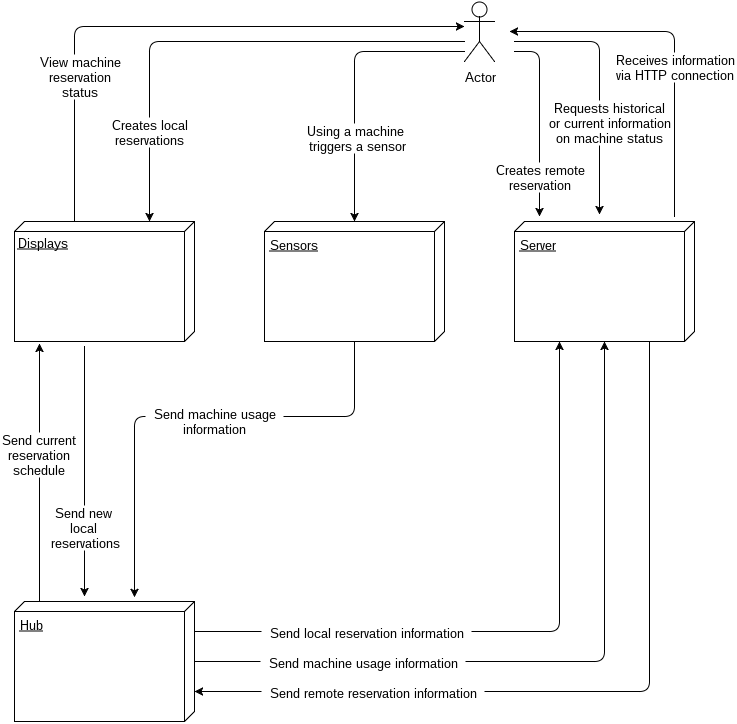
\includegraphics[width=\textwidth]{uml/general_overview.png}
    \caption{UML Diagram of the System Overview}
    \label{fig:general_overview}
\end{figure}

\section{Current Project Status}	

The team is currently working on developing the four major hardware requirement areas outlined in section 3.2. The work is as follows:

\subsection{Sensors}
The team has successfully loaded custom code on the TI SensorTags and is able to read and store this output. There is currently work being done that uses signal processing to analyze the output and determine whether a machine is in use or not. The team is also able to turn off selected sensors on the SensorTag.

\subsection{Displays}
The team has received all the necessary equipment to work with the displays, as well as the displays themselves, but has not yet started working with the on-machine display development. This is primarily because it is seen as a secondary function when compared to retrieving information from the sensors. There is, however, development for displaying information for all the machines. This will be discussed more in section 5.4.

\subsection{Hub}
The team has developed a system that is able to send rudimentary information about the current status of machines from the hub to the server. It is also able to retrieve information from the server and then get the packets ready to send onward to the sensors and displays. All of the logic is abstracted out so that whatever wrinkles are found during the development of the sensors and displays will be able to be on the outside of the hub development. This has allowed this development to continue parallel to the sensor and display development.

\subsection{Server}
The server's two main goals currently have functioning prototypes. There is a database implemented that can store users, machines, and their relationships, as well as a database model that abstracts out the implementation for other services to be able to use. There is a website that is currently being implemented that interfaces with the database model to get information specified by the requirements. This has placeholders for each of the important pages, along with guidelines for what each page is required to do.

\subsection{Summary}
The team has made progress that is on schedule with what is planned for the semester. The main goals left for the team are to start connecting each of the different areas, adding functionality on the user end, and implementing the on-machine displays.

\end{document}
